\chapter{Modellierung}
\label{sec:modellierung}
Im mathematischen Modell werden die Anforderungen aus der Trainingswissenschaft in das Format der Constraint Programmierung übersetzt. Die Modellierung löst jeden Monat (=28 Tage) gesondert und berechnet die Trainingseinheiten für diesen Zeitraum. Dauer, Methode und Leistungsbereiche charakterisieren eine Einheit. Später werden die Mesozyklen dann zu einem Makrozyklus verbunden.

\section{Verfahrensweise}
\label{sec:modellierung:uebersicht}
\begin{figure}[htb]
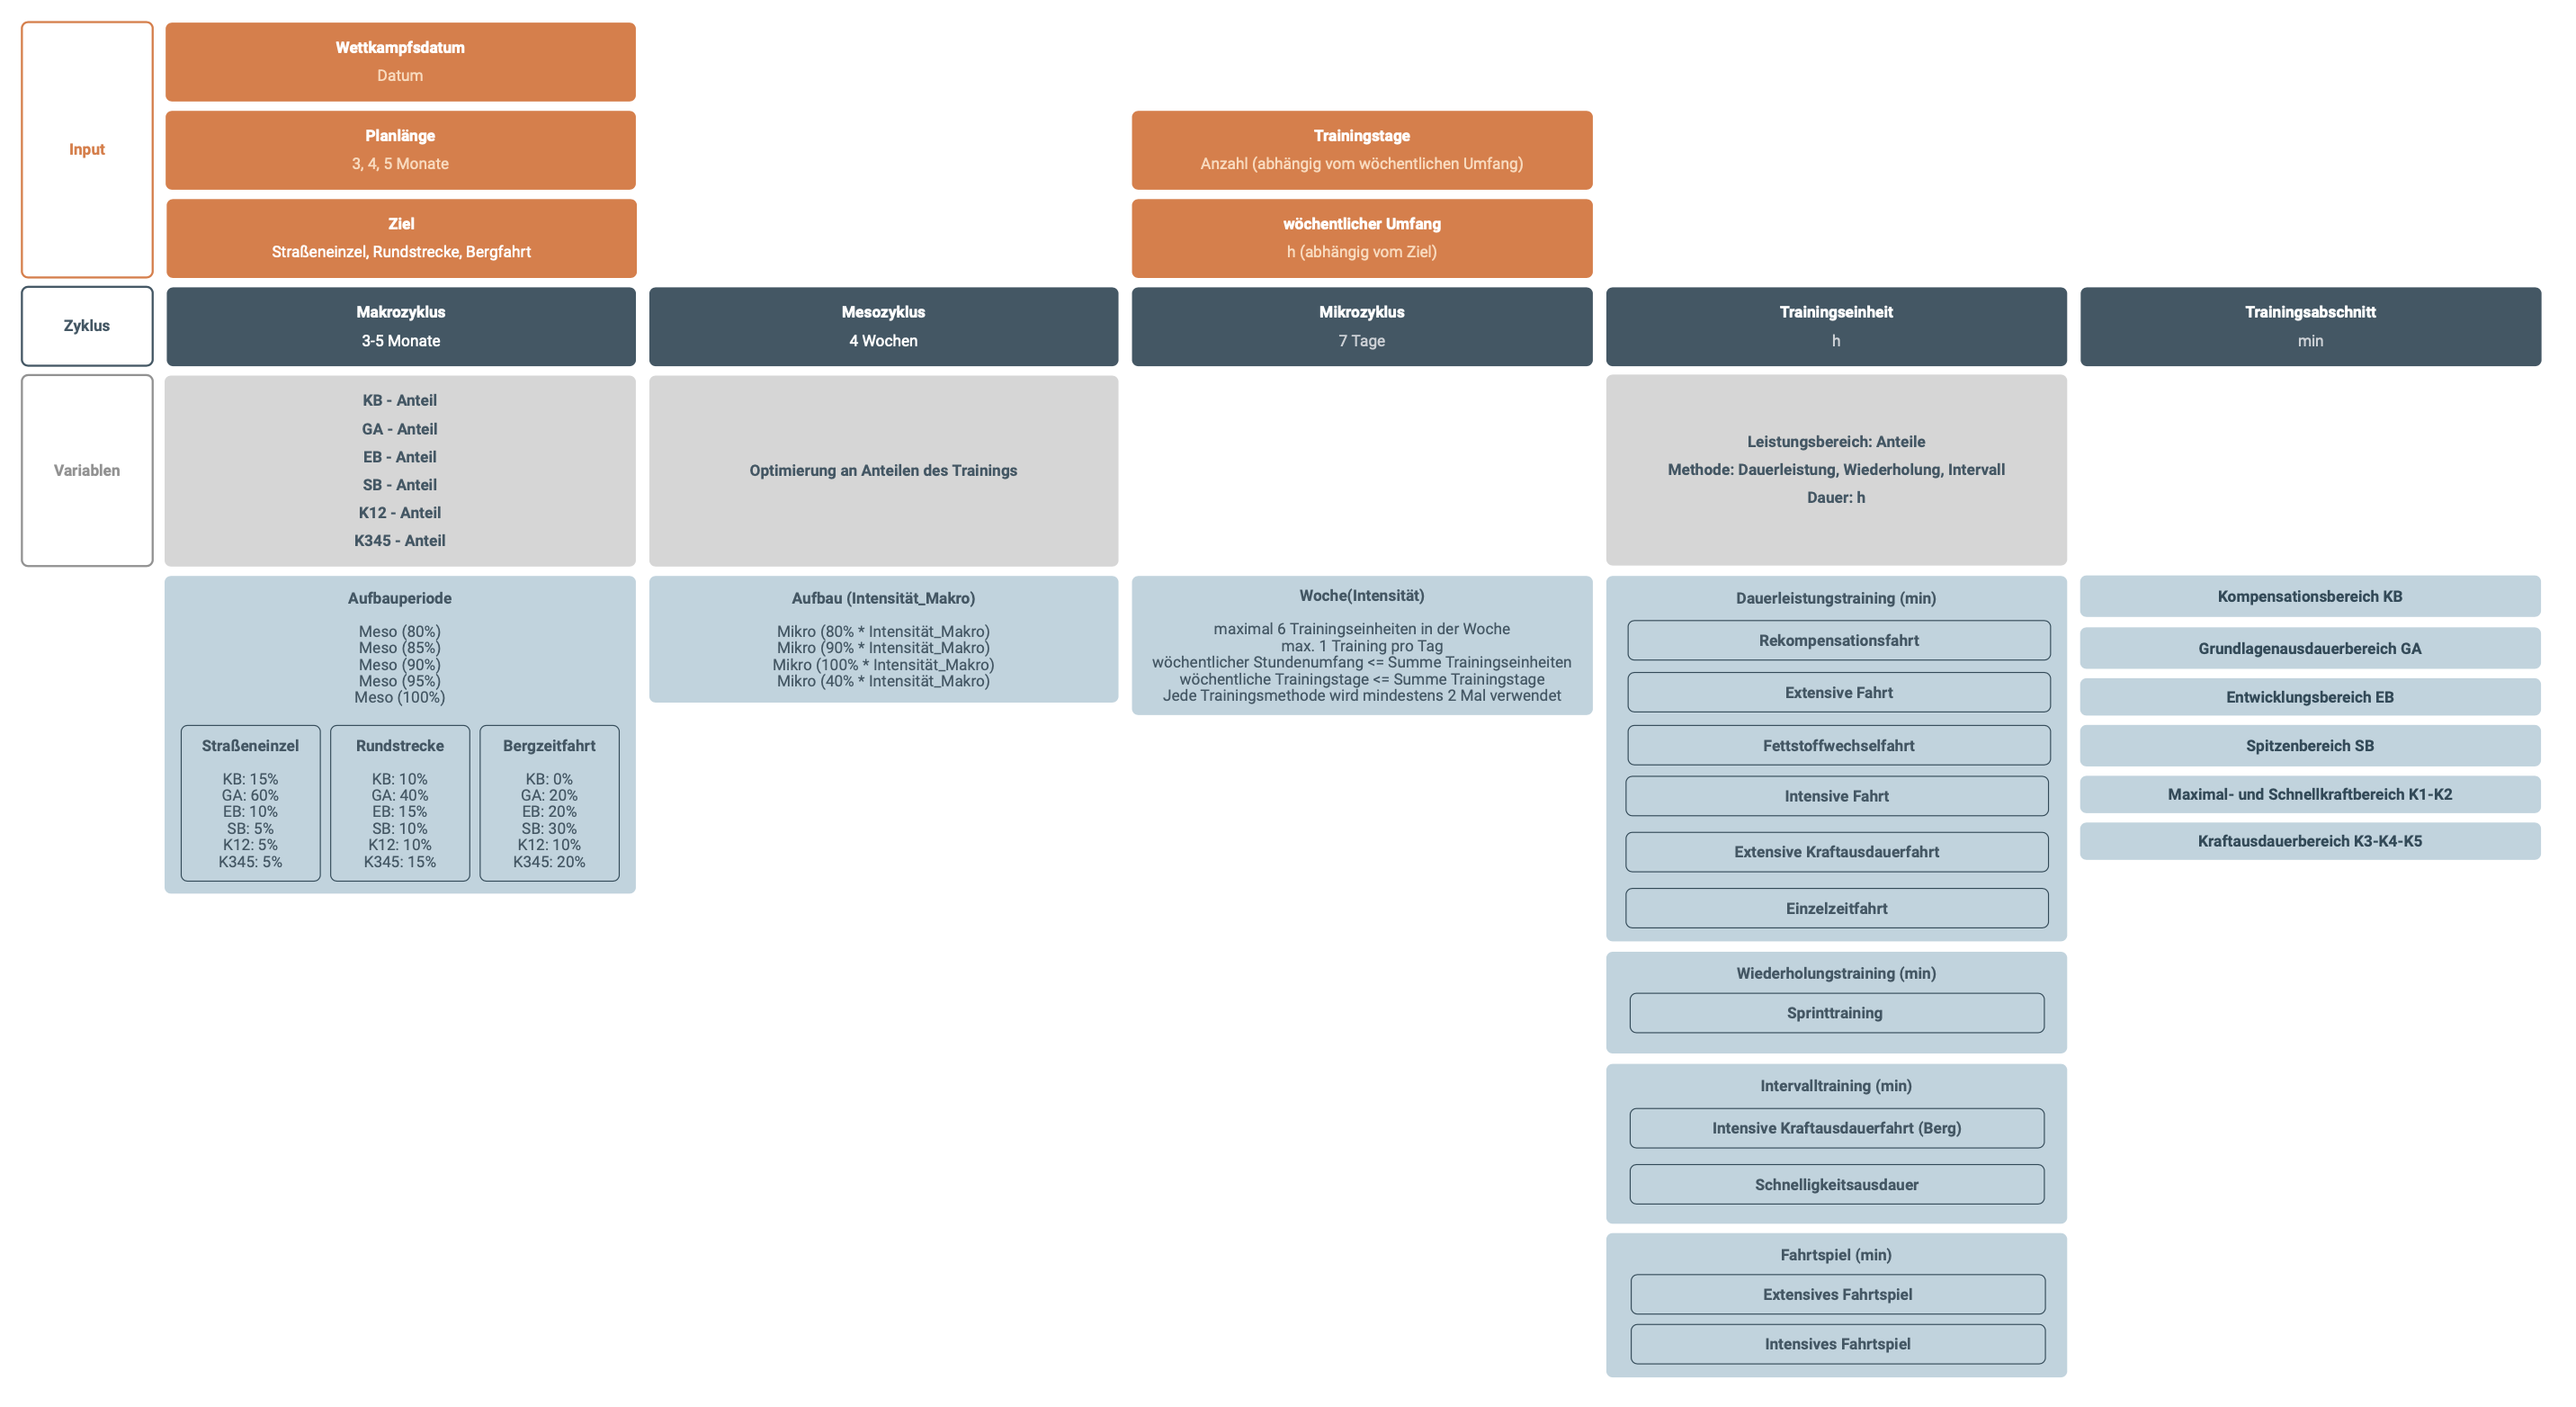
\includegraphics[width=\textwidth]{gfx/modellierung.png}
\caption{Schema aus Makro-, Meso- und Mikrozyklen}
\label{fig:modellierung:schema}
\end{figure}

\begin{enumerate}
    \item Trainingsziel und Plandauer bestimmen
    \item Jeden Monat des Trainingplans einzeln lösen
    \item Die vier Wochen des Mesozyklus progressiv gestalten mit einer 3:1 Periodisierung
    \item Constraints auf Ebene der Hierarchie definieren 
    \item Solver parallelisiert für jeden Mesozyklus starten
    \item Trainingseinheiten aus den Mesozyklen zu einem Trainingsplan zusammensetzen
\end{enumerate}

\section{Designentscheidungen}
Im ersten Ansatz der Modellierung eines Trainingsplans wurden kein kombinatorischer Grundgedanke verfolgt. Statt eines Pools an validen Trainingseinheiten, definierte das System die Charakteristika einer Trainingsmethode. Die Schwierigkeit ist jedoch die vielen Einzelfälle und Ausnahmen präzise genug abzudecken ohne ein sehr unübersichtliches Constraint-System zu erhalten. Besonders im Hinblick auf die Erweiterung und Skalierbarkeit scheiterte dieser Versuch. Stattdessen wird das Problem als kombinatorische Problem betrachet, das die einzelnen Elemente -- als Verteilung der Trainingseinheiten -- dynamisch definiert. \par
Des Weiteren wurde von einer Modellierung auf Basis von Kraft, Ausdauer und Schnelligkeitsanteilen abgesehen. In diesem Fall wären Schätzungen an zwei Stellen vonnöten. Erst müssen für die Trainingseinheiten die drei Bereiche festgelegt werden und dann, wie auch in der aktuellen Modellierung, die Gewichtung in Abhängigkeit der Wettkampfsdisziplin. Mit Definition einer Trainingseinheit über die Leistungsbereiche selbst, kann die Abschätzung an einer Stelle gebündelt werden.\par
Die Optimierung auf Ebene der Mesozyklen erlaubt der Verteilung und Variation genug Spielraum. Die Gefahr einer wochenweisen Optimierung ist, dass es eine Lösungsinstanz gibt, die für alle Wochen in ähnlicher Form verwendet wird. Die Variation lässt sich damit nicht genügend steuern. Anhand der monatlichen Kapselung wirkt man der Monotonie entgegen und kann dennoch in Teilprobleme zerlegt werden.

\section{Model}
\subsection{Konstanten}
In der Modellierung betrachten wir Konstanten gesondert. Diese Größen sind in jeder Lösungsinstanz relevant aber vor der Modellierung fest bestimmt.

$maxminutes$ legt die Beschränkung der Trainingsminuten einer Woche festgesetzt.
\[ maxminutes \in [0, 1200] \]

Analog dazu gibt es auch eine Begrenzung der Trainingstage einer Woche. Die Anforderung an mindestens einen Regenerationstag ist hier umgesetzt, da die Trainingstage nicht 7 Tage betragen können.
\[ maxdays \in [2, 6] \]

Input Trainingsziel
\[ kb, ga, eb, sb, k1, k4 \in [0, 100] \]

\subsection{Variablen}
Unter den Variablen der Modellierung versteht man die veränderlichen Größen. Die endlichen Wertebereiche sind möglichst präzise zu wählen. Eine Lösungsinstanz definiert die Belegung der Variablen mit konkreten Werte.

\textbf{Dauer einer Einheit} \\[0.2em]
Variable für die Dauer der Trainingseinheit an Tag $i$ in Minuten. Es wird für einen Tag eine maximale Trainingszeit von 6 Stunden angesetzt.
\begin{equation} 
    \forall i \in [1, 28], \text{duration}_i = [\![0, 360]\!] \end{equation} 
\textbf{Trainingsmethode einer Einheit} \\[0.2em]
Variable für die Trainingsmethode der Trainingseinheit an Tag $i$. Für Tage ohne Trainingseinheit wird die Methode \textit{PAUSE} eingeführt.
\begin{equation} 
    \forall i \in [1, 28], \text{method}_i = \{\text{PAUSE, DL, FS, IV, WH}\}
\end{equation} 
\textbf{Leistungsbereiche einer Einheit} \\[0.2em]
Variable für die Minuten je Belastungsbereich an Tag $i$. Die maximale Trainingszeit gilt hier gleichermaßen.
\begin{equation} 
\begin{array}{c}
    \forall i \in [1, 28], \text{kb}_i = [\![0, 360]\!] \\
    \forall i \in [1, 28], \text{ga}_i = [\![0, 360]\!] \\
    \forall i \in [1, 28], \text{eb}_i = [\![0, 360]\!] \\
    \forall i \in [1, 28], \text{sb}_i = [\![0, 360]\!] \\
    \forall i \in [1, 28], \text{k1}_i = [\![0, 360]\!] \\
    \forall i \in [1, 28], \text{k4}_i = [\![0, 360]\!] \\
\end{array}
\end{equation} 
\subsection{Constraints}
\textbf{Diskretisierung der Trainingseinheiten} \\[0.2em]
Die Trainingseinheiten werden bei ihrer Länge auf viertelstündliche Abschnitte diskretisiert. 
\begin{equation}
    \forall i \in [1, 28], min_i \mod 15 = 0
\end{equation} 

\textbf{Diskretisierung der Trainingsbereiche} \\[0.2em]
Die Trainingsbereiche einer Einheit können in fünf Minuten Abschnitten festgesetzt werden.
\begin{equation}
\begin{array}{c}
    \forall i \in [1, 28], kb_i \mod 5 = 0 \\
    \forall i \in [1, 28], ga_i \mod 5 = 0 \\
    \forall i \in [1, 28], eb_i \mod 5 = 0 \\
    \forall i \in [1, 28], sb_i \mod 5 = 0 \\
    \forall i \in [1, 28], k1_i \mod 5 = 0 \\
    \forall i \in [1, 28], k4_i \mod 5 = 0 \\
\end{array}
\end{equation}

\textbf{Variation der Trainingsmethoden} \\[0.2em]
Um die Variation der Trainingsmethoden zu garantieren, wird verlangt, dass jede Trainingsmethode mindestens zwei Mal verwendet wird. Da auf Ebene der Mesozyklen modelliert wird und somit je für 28 Tage ist diese Bedingung erfüllbar. Die Mindestanzahl der Tage mit Training ist 8 und somit ist die Bedingung auch bei der Mindestanzahl von 2 Trainingstagen erfüllbar. $\{DL, FS, IV, WH\}$
\begin{equation} 
    \forall m \in ,|\{method_i = m | i \in [1, 28]\}| \geq 2
\end{equation} 

\textbf{Limitierung des wöchentlichen Stundenumfangs} \\[0.2em]
Summe der Trainingsstunden unter wöchentlichem Umfang
\begin{equation}
    \forall i = k * 7 + 1, k \in Z, \sum_{i}^{i+6} \text{duration}_i \leq max_{hours} 
\end{equation}
\begin{equation}
    \forall i \in \{ i = k * 7 + 1, k \in Z \}, \sum_{i}^{i+6} \text{duration}_i \leq max_{hours}
\end{equation}

\textbf{Limitierung der wöchentlichen Trainingstage} \\[0.2em]
Summe der Trainingstage unter wöchentlichem Maximalwert
\begin{equation}
    \forall i = k * 7 + 1, k \in Z, \sum_{i}^{i+6} \text{day}_i \leq max_{days}
\end{equation}

\textbf{Definition von Pause} \\[0.2em]
Ist an einem Tag die Trainingsdauer auf Null gesetzt, entspricht das einer Pause im Trainingsplan. Die Pause als Trainingsmethode umzusetzen erlaubt es, immer 28 Tage zu modellieren.
\begin{equation}
    method_i = \text{PAUSE} \Leftrightarrow minutes_i = 0
\end{equation}

\textbf{Menge der validen Trainingseinheiten} \\[0.2em]
Wie bereits in Abschnitt \ref{grundlagen:methoden} definiert, werden die möglichen Trainingseinheiten einer Trainingsmethode als Menge vorgegeben. Exemplarisch am Fahrtspiel gelten dann folgende Bedingungen für die geordnete Menge $ranges_i = (kb_i, ga_i, eb_i, sb_i, k1_i, k4_i)$. Die vollständige Modellierung befindet sich im Anhang \ref{anhang:code:modell}.
\begin{equation}
    (method_i = \text{Fahrtspiel})\Rightarrow t_i = \begin{array}{c}
            (0, [\![60, 240]\!], [\![60, 240]\!], 0, 0, 0) \\ 
        \vee (0, [\![60,180]\!], [\![60, 180]\!], [\![60, 180]\!], 0, 0)
    \end{array}
\end{equation}

\subsection{Optimierung}
Die Modellierung berechnet die Summe der Trainingsminuten in den verschiedenen Belastungsbereichen. Die Distanz dieser zu der kalkulierten Vorgabe wird summiert und als Abweichung des Modells festgelegt. Mithilfe dieser Größe wird die Güte einer Lösungsinstanz quantifiziert. Das Modell strebt bei der Lösung die Minimierung dieses Wertes an.
\begin{equation}
    \text{minimize} \sum_{m\in M} |\text{target}_m - \text{sum}_m|
\end{equation} 

% Basierend auf dem Trainingsziel werden die Zyklen mit spezifischer Gewichtung gestaltet. Dabei sind Belastungs und Regenerationsphasen einzuplanen. Danach fließt in der Phase der konkreten Trainingsplanung die Anforderung und das individuelle Belastungsprofil des Sportlers ein. Regenerationsphasen müssen berücksichtigt werden. 
% In der letzten Phase werden die konkreten Trainingseinheiten festgelegt. Diese beinhalten sowohl Trainingsmethoden, als auch Intensität und Dauer der Belastungen. 
% Diese Arbeit behandelt ausschließlich die initiale Erstellung eines Trainingsplans. Es erfolgt keine Trainingssteuerung durch Dokumentation oder Kontrolle.